\documentclass{/home/janmebows/Documents/LatexTemplates/myassignment}
\title{Topic C Assignment 3}

\begin{document}

\maketitle
\begin{enumerate}
	\item \begin{enumerate}
		\item 
		\begin{align*}
			\epsilon \frac{d^2y}{dx^2} + (\cosh x) \frac{dy}{dx} - y= 0\\
		\end{align*}
		With $y(0)=y(1)=1$
		To leading order:
		\[y = y_0 + \bigo(\epsilon)\]
		\begin{align*}
			(\cosh x)\frac{dy_{0,out}}{dx} - y_0 = 0\\
			\frac{1}{y_{0,out}}\frac{dy_{0,out}}{dx} = \sech x \\
			\log y_{0,out} = 2\arctan\left(\tanh x/2\right)\\
			\boxed{y_{0,out} = a\exp\{2\arctan\left(\tanh x/2\right)\}}
		\end{align*}
		For the boundary conditions:
		
		%answer looks like utter crap
		Let $x = x_* + \delta_1 X$, and $y = \delta_2 Y$
		\begin{align*}
			\epsilon \frac{\delta_2^2}{\delta_1^2}\frac{d^2Y}{dX^2} + (\cosh(x_* + \delta_1 X))\frac{\delta_2}{\delta_1} \frac{dY}{dX} - \delta_2 Y= 0\\
		\end{align*}
		With BCs $\delta_2 Y(0) = \delta_2 Y(1) = 1$ Hence $\delta_2 = 1$.
		\[\epsilon \frac{1}{\delta_1}\frac{d^2Y}{dX^2} + (\cosh(x_* + \delta_1 X))\frac1{\delta_1} \frac{dY}{dX} - Y= 0\]
		Expand the $\cosh$ term:
		\begin{align*}
			\cosh (x_*+\delta_1 X) &= \cosh(x_*)\cosh(\delta_1X) + \sinh(x_*)\sinh(\delta_1X)\\
			&=\sinh(x_*)\sum_{i=0}^\infty \frac{(\delta_1 X)^{2i+1}}{(2i+1)!}   + \cosh(x_*)\sum_{i=0}^\infty \frac{(\delta_1 X)^{2i}}{(2i)!}\\
			&= \sinh(x_*)\left(\delta_1 X\right) + \cosh(x_*) + \bigo(\epsilon^2) 
		\end{align*}
		Noting that $x^* = 0$ or $x^* =1$.
		\[\epsilon \frac{1}{\delta_1}\frac{d^2Y}{dX^2} + (\sinh(x_*)\left(\delta_1 X\right) + \cosh(x_*))\frac1{\delta_1} \frac{dY}{dX} - Y= 0\]
		\[\epsilon\frac{d^2Y}{dX^2} +  \delta_1 X \sinh(x_*)\frac{dY}{dX} + \cosh(x_*)\frac{dY}{dX} - \delta_1 Y= 0\]
		Hence $\delta_1 = \epsilon$

		If $x^* = 0$ (which a numerical solution says is true)

		\begin{align*}
			\frac{d^2Y}{dX^2} + X\sinh(0) \frac{dY}{dX} - Y = 0\\
			\frac{d^2Y}{dX^2} - Y = 0\\
			Y = Ae^{X} + Be^{-X}
		\end{align*}
		$Y(0) = 1$:
		\begin{align*}
			Ae^{0} + Be^{0} = 1\\
			A+B =1\\
			B = 1-A
		\end{align*}
		Hence
		\[\boxed{Y = Ae^{X} + (1-A)e^{-X}}\]
		And the outer solution becomes
		\begin{align*}
			y_{0,out}(1) = 1 = a\exp\{2\arctan\left(\tanh 1/2\right)\}\\
			a = \exp\{-2\arctan\left(\tanh 1/2\right)\}
		\end{align*}
		\[\boxed{y_{0,out} =\exp\{2\arctan\left(\tanh x/2\right) -2\arctan\left(\tanh 1/2\right) \} } \]

		Matching
		\begin{align*}
			\lim_{x\to 0} y_0(x) &= \lim_{X \to \infty} Y_0(X)\\
			a\exp\{\arctan(\tanh(0))\} &= Ae^{\infty} + (1-A)e^{-\infty}\\
		\end{align*}

		\begin{align*}
			y_{comp} &= y_{in} + y_{out} - y_{overlap}\\
			&=
		\end{align*}


		\begin{align*}
			y_{0,out}(0) = 1 = a\exp\{2\arctan\left(\tanh 0\right)\}\\
			a \exp^0 = 1 \\
			a = 1
		\end{align*}



		% \begin{align*}
		% 	\frac{d^2Y}{dX^2} + X\sinh(x_*) \frac{dY}{dX} - Y = 0
		% \end{align*}

		\begin{align*}
			\lim_{x\to 1} y_0(x) &= \lim_{X \to -\infty} Y_0(X)\\
		\end{align*}

		\item WKB ansatz solution for
		\[\epsilon \frac{d^2y}{dx^2} + (\cosh x) \frac{dy}{dx} - y= 0\]
		\[y(x) \sim \sum_{n=0}^\infty u_n(x) \epsilon^n + e^{-F(x)/\epsilon} \sum_{n=0}^\infty v_n(x) \epsilon^{n}\] 
		Leading order:
		\begin{align*}
			y \sim u_0 + e^{-F/\epsilon} v_0\\
			y' \sim u_0' + e^{-F/\epsilon} v_0' - \frac{F'}{\epsilon} e^{-F/\epsilon}(v_0 + \epsilon v_1 + \hdots)\\
			y'' \sim u_0'' + e^{-F/\epsilon} v_0'' - 2\frac{F}{\epsilon} v_0' + \left(\frac{F'}{\epsilon}\right)^2 e^{-F/\epsilon} \left(v_0 + \epsilon v_1 + \ldots\right) - \frac{F''}{\epsilon} e^{-F/\epsilon} v_0
		\end{align*}
		So the equation becomes:
		\begin{align*}
			\epsilon \frac{d^2y}{dx^2} + (\cosh x) \frac{dy}{dx} - y= 0\\
			\epsilon\left(u_0'' + e^{-F/\epsilon} v_0'' - 2\frac{F}{\epsilon} v_0' + \left(\frac{F'}{\epsilon}\right)^2 e^{-F/\epsilon} \left(v_0 + \epsilon v_1 + \ldots\right) - \frac{F''}{\epsilon} e^{-F/\epsilon} v_0\right)\\
			+ \cosh x\left(u_0' + e^{-F/\epsilon} v_0' - \frac{F'}{\epsilon} e^{-F/\epsilon}(v_0 + \epsilon v_1 + \hdots)\right) - u_0 + e^{-F/\epsilon} v_0 =0\\\\
			\epsilon u_0'' + \epsilon e^{-F/\epsilon} v_0'' - 2F v_0' + \frac{F'^2}{\epsilon} e^{-F/\epsilon} \left(v_0 + \epsilon v_1 + \ldots\right) - F'' e^{-F/\epsilon} v_0\\
			+ \cosh x\left(u_0' + e^{-F/\epsilon} v_0' - \frac{F'}{\epsilon} e^{-F/\epsilon}(v_0 + \epsilon v_1 + \hdots)\right) - u_0 + e^{-F/\epsilon} v_0 =0
		\end{align*}
		\begin{align*}
			\bigo(1): 0 &= -2F v_0' +(\cosh x)u_0' - u_0\\
			\bigo(e^{-F(x)/\epsilon} \epsilon^{-1}) : 0&=\left[F'- \cosh x\right]\\
			\bigo(e^{-F(x)/\epsilon}) : 0&=
		\end{align*}


		\item First rewrite the BVP in a nicer format
		\[\frac{d^2y}{dx^2} + \frac{1}{\epsilon} \left(\cosh x\frac{dy}{dx} - y\right) = 0\] 
		Figure~\ref{fig:q1}
	\begin{figure}[tb]
		\centering
		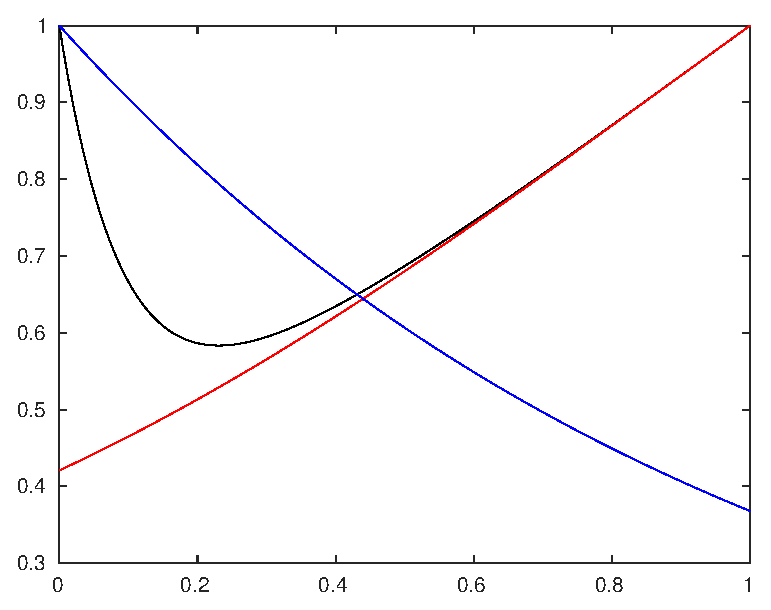
\includegraphics{TopicCA3Q1}
		\caption{Comparison of Numerical, WKB and Composite solutions}
		\label{fig:q1}
	\end{figure}
	\end{enumerate}



	\item 
	%Find leading order solutions to
	\[\epsilon \frac{d^2y}{dx^2} + x\frac{dy}{dx} + xy =0\]
	With $y(-2)=-4$ and $y(2) =2$, $\epsilon \to 0$ over $-2\leq x \leq 2$. There is an internal boundary layer shown via the numerical solution, in figure~\ref{fig:q2}

	The right outer solution $y_R$ with $y_R(2) = 2$ to leading order:
	\begin{align*}
	xy_{R0}' + xy_{R0} = 0\\
	y_{R0}' + y_{R0} = 0\\
	y_{R0} = Ae^{-x}
	\end{align*}
	And applying the boundary condition:
	\begin{align*}
		y_{R0}(2) = Ae^{-2} = 2\\
		A = 2e^2
	\end{align*}

	\[\boxed{y_{R0} = 2e^2e^{-x} } \]
	
	The left outer solution $y_L$ with $y_L(-2) =-4$
	\begin{align*}
	y_{L0} = Be^{-x}\\
	y_{L0}(-2) = Be^{-2} = -4\\
	B = -4e^{-2}
	\end{align*}
	Hence
	\[\boxed{y_{L0} = -4e^{-2}e^{-x} } \]

	For the inner solution $x = x_* + \delta_1 X$, and $y = \delta_2 Y$. Since the boundary conditions don't include $\epsilon$, $\delta_2 =1$.
	\begin{align*}
		\epsilon \frac{d^2y}{dx^2} + x\frac{dy}{dx} + xy =0\\
		\epsilon \frac{1}{\delta_1^2}\frac{d^2Y}{dX^2} + (x^* + \delta_1X)\frac{1}{\delta_1}\frac{dY}{dX} + (x^* +\delta_1 X)Y =0\\
		\epsilon \frac{d^2Y}{dX^2} + \delta_1 (x^* + \delta_1 X)\frac{dY}{dX} + \delta_1^2 (x^* + \delta_1X)Y = 0\\
		\epsilon \frac{d^2Y}{dX^2} + \delta_1 x^*\frac{dY}{dX} + \delta_1^2 X\frac{dY}{dX} + \delta_1^2 x^*Y+ \delta_1^{3}XY = 0\\
		\epsilon \frac{d^2Y}{dX^2} + \delta_1 x^*\frac{dY}{dX} + \delta_1^2\left( X\frac{dY}{dX} + x^*Y\right)+ \delta_1^{3}XY = 0\\
	\end{align*}
	
	%%%%ALl this is wrong
	Balances:
	\begin{itemize}
		\item $\epsilon \frac{d^2Y}{dX^2} \sim \delta_1 x^*\frac{dY}{dX}$ Hence $\delta_1 \sim \epsilon$, this is reasonable since the rejected terms will be $\bigo(\epsilon^2)$ and $\bigo(\epsilon^3)$ both of which are negligible.
		\item $\epsilon \frac{d^2Y}{dX^2} \sim - \delta_1^2\left( X\frac{dY}{dX} + x^*Y\right) $ giving $\delta \sim \sqrt{\epsilon}$ neglecting terms of order $\epsilon^{1/2}$ and $\epsilon^{3/2}$. But $\epsilon^{1/2}\gg \epsilon$ so this is a contradiction. 
		\item $\epsilon \frac{d^2Y}{dX^2} \sim - \delta_1^{3}XY $ with $\delta_1 \sim \epsilon^{1/3}$, meaning we have neglected the $\epsilon^{1/2}$ and $\epsilon^{1/3}$ terms in favour of $\epsilon$. This is a contradiction since $\epsilon^{1/3} \gg \epsilon$

	\end{itemize}
	Hence take $\delta_1 = \epsilon$

	To leading order:
	\begin{align*}
	\frac{d^2Y_0}{dX^2} = - x^*\frac{dY_0}{dX}\\
	V' = -x^* V\\
	\implies V = ae^{-x^* X}\\
	\implies Y_0 =a_0 e^{-x^* X} +b
	\end{align*}
	We have to match this to the left and right solutions

	Start with the right:
	\begin{align*}
		\lim_{x\to x^*} y_{R0}=\lim_{X\to \infty} Y_0(X)\\
		\lim_{x\to x^*} 2e^2e^{-x}  = \lim_{X\to \infty} a_0 e^{-x^* X} +b
	\end{align*}
	The left:
	\begin{align*}
		\lim_{x\to x^*} y_{L0}=\lim_{X\to -\infty} Y_0(X) \\
		\lim_{x\to x^*} -4e^{-2}e^{-x} = \lim_{X\to -\infty} a_0 e^{-x^* X} +b
	\end{align*}


	\begin{figure}[tb]
		\centering
		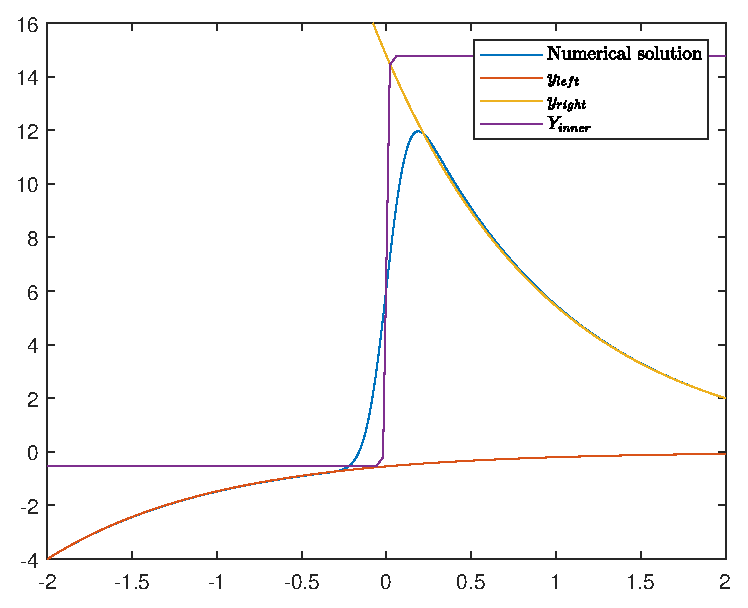
\includegraphics{TopicCA3Q2}
		\caption{Caption here}
		\label{fig:q2}
	\end{figure}
\end{enumerate}
\section*{Matlab Code}
\lstinputlisting{AppTopicCA3.m}

\clearpage
\includepdf[pages=1-]{PA_2019_A3.pdf}

\end{document}